\section{Galaxy Classification}


In this section we will attempt to implement a logistic regression algorithm to classify galaxies into two classes, ellipticals and spirals, using four parameters:

\begin{itemize}
    \item $\kappa_{\mathrm{co}}$, which indicates how much a galaxy is dominated by ordered rotation
    \item A color estimate (higher is redder, and therefore contains older stars)
    \item A measure of how extended the galaxy is
    \item Flux of an emission line tracing the star formation rate
\end{itemize}

We start by preprocessing all of the features by scaling them to have zero mean and unit standard deviation. This is implemented for each feature $f_i$ separately as

\begin{equation}
    f_{i, \mathrm{scaled}} = \frac{f_i - \mu_i}{\sigma_i}
\end{equation}

To get a sense of how each of our features is distributed, we plot their histograms in Figure \ref{fig:feat_dist}, and present the first ten samples below.

\lstinputlisting[caption={Scaled feature values for the first ten entries of the galaxy dataset}, lastline=10]{results/scaled_features.txt}
\lstinputlisting[caption={Code to make the histograms in Figure \ref{fig:feat_dist}}, linerange={15-36}]{plotting.py}
\lstinputlisting[caption={Code for the feature preprocessing and plotting.}, linerange={6-36}]{classification.py}

\begin{figure}
    \centering
    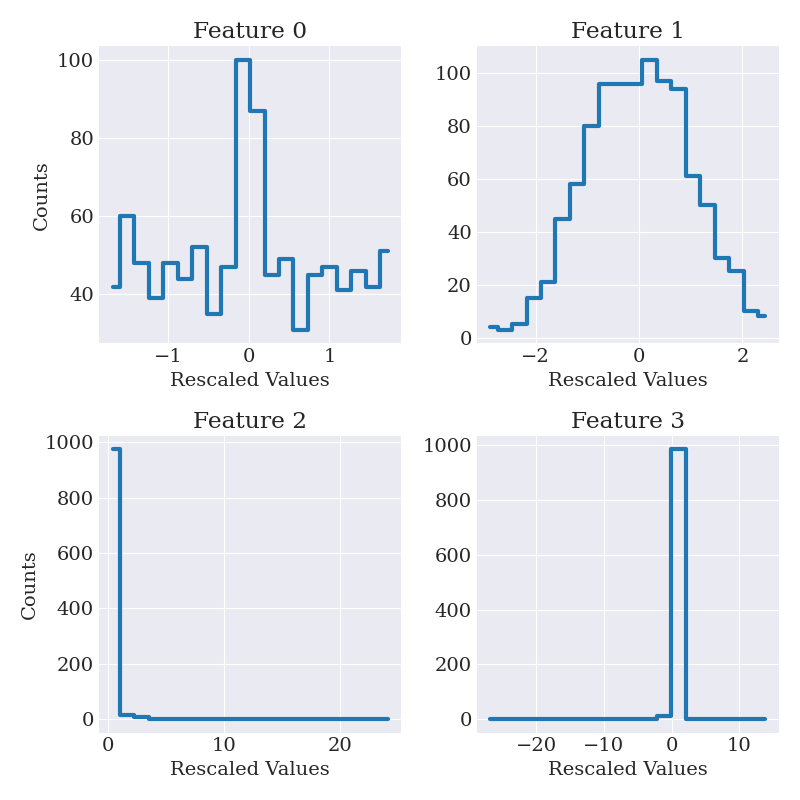
\includegraphics[width=0.8\textwidth]{results/scaled_features_dist.png}
    \caption{Distributions of the scaled features used for the classification algorithms in this section.}
    \label{fig:feat_dist}
\end{figure}

It is immediately noticable that while most values for features 2 and 3 lie around 0, there are outliers at extremely high values. This is less true for feature 0 which shows a peak at 0 and has a relatively constant distribution in its wings. Feature 1 appears to be nicely distributed close to a Gaussian. Due to the few outliers in features 2 and 3 we will limit ourselves to the 2\% and 98\% percentiles for plotting in the rest of this work to better highlight the variations in the regions where the bulk of the datapoints reside. Ofcourse we do not discard these points for the training process.

\subsection{Two Feature Combinations}

\lstinputlisting[caption={Code for fitting the classification algorithm and computing the F1 score for each two feature combination and both minimization types}, linerange={38-113}]{classification.py}
\lstinputlisting[caption={Logistic Regresion, Confusion Matrix and F1 Score code}, firstline={197}]{algorithms.py}
\lstinputlisting[caption={Code for 'smarter' function minimization}]{minimization.py}

We begin by investigating how well the logistic regression algorithm is able to predict the galaxy class if it is only provided with two of the four available features. We do this by running the algorithm by each of the six possible combinations of two features and investigating the resulting loss values. In each case we also include a bias feature consisting of only ones. As an extra test we also look at the differences between using a constant step size $\eta = 0.1$ and using line minimization using golden section search to discover the minimum. We show the resulting loss curves, the evolution of the loss value as a function of iteration, in Figure \ref{fig:losscurve_stepsize} for the learning rate method and in Figure \ref{fig:losscurve_linemini} for the line mininimization method. 

\begin{figure}
    \centering
    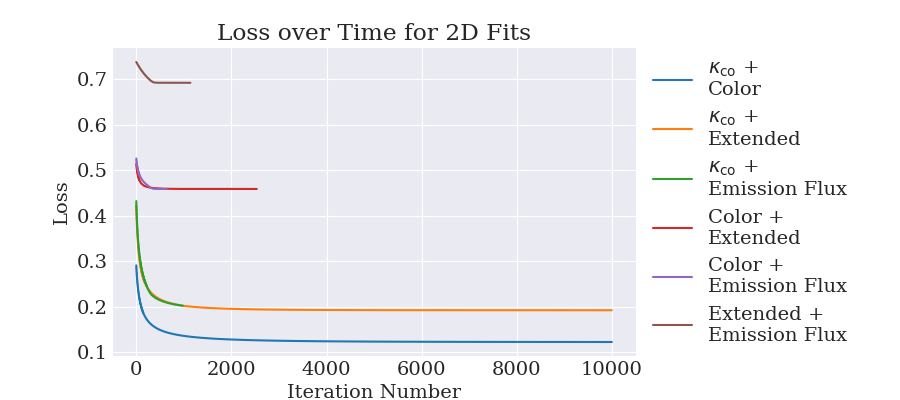
\includegraphics[width=\textwidth]{results/2d_fit_losses_constant_step.png}
    \caption{Loss value as a function of iteration number for each of the six possible combinations of two out of four features using logistic regression and a constant step size as minimization method.}
    \label{fig:losscurve_stepsize}
\end{figure}

\begin{figure}
    \centering
    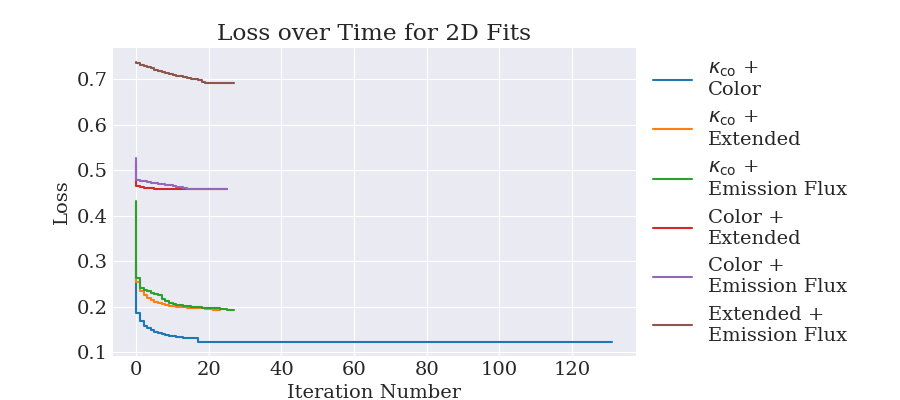
\includegraphics[width=\textwidth]{results/2d_fit_losses_line_minim.png}
    \caption{Loss value as a function of iteration number for each of the six possible combinations of two out of four features using logistic regression and line minimization as minimization method.}
    \label{fig:losscurve_linemini}
\end{figure}

We can see that under both minimization methods, all loss values converge to approximately the same values. However line minimization converges $\sim 100 - 1000$ times faster than using a learning rate of $0.1$. From these plots we can gather that the combination of $\kappa_{\mathrm{CO}}$ and color estimate is the best combination of parameters to estimate galaxy class. Meanwhile, the extended measure and the flux of the emission line tracing star formation rate appear to be a very bad combination of predictors. To get a better grasp of the distribution of the features, and the prediction capablity of our models, we plot all six of the two dimensional combinations of distributions of the features coloured by their galaxy class together with the decision boundary as learned by the logistic regression model in Figure \ref{fig:2d_line_minim_scatter}. We only plot the results of the line minimization method here.


\begin{figure}
    \centering
    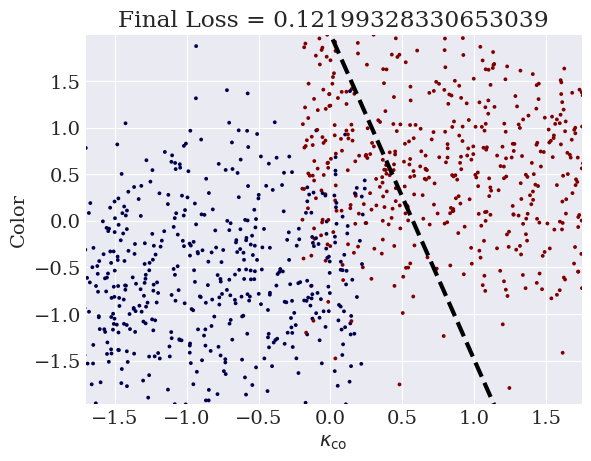
\includegraphics[width=0.48\textwidth]{results/2d_fit_line_minim_kappa_color.png}
    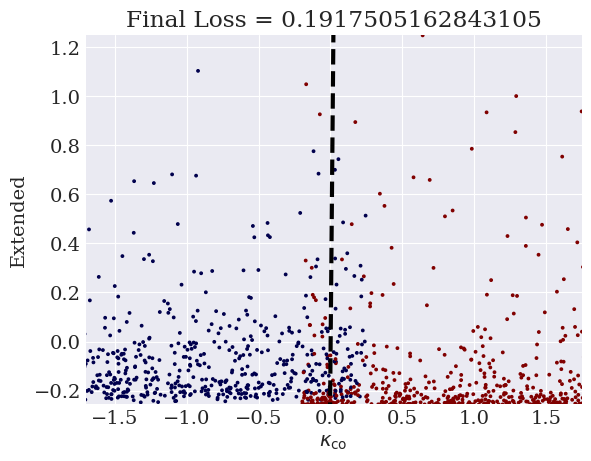
\includegraphics[width=0.48\textwidth]{results/2d_fit_line_minim_kappa_extended.png}
    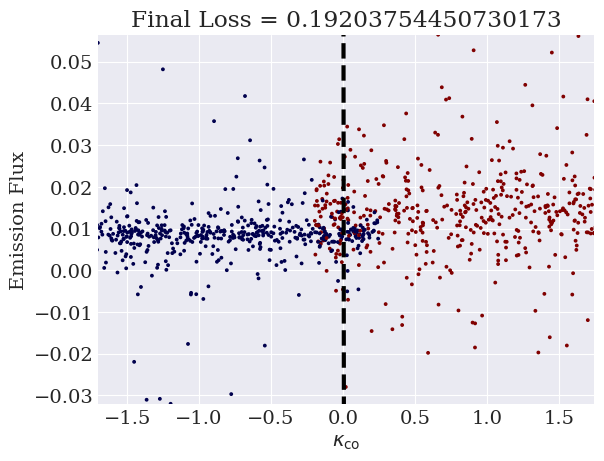
\includegraphics[width=0.48\textwidth]{results/2d_fit_line_minim_kappa_emission_flux.png}
    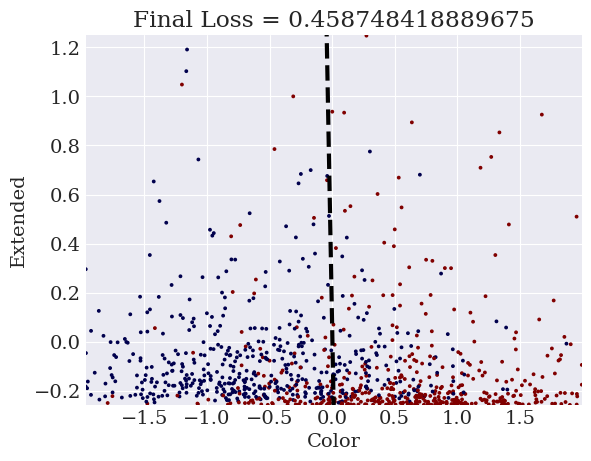
\includegraphics[width=0.48\textwidth]{results/2d_fit_line_minim_color_extended.png}
    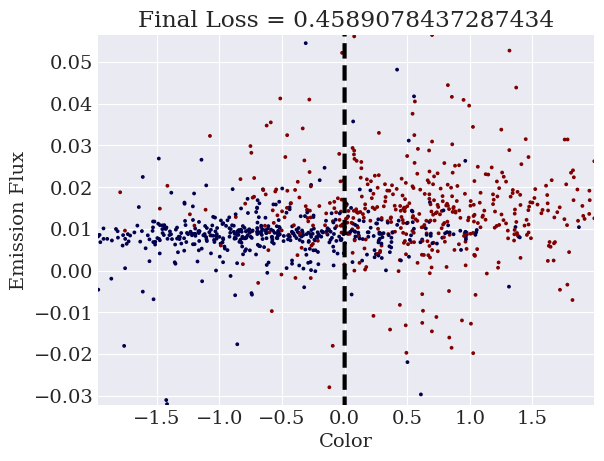
\includegraphics[width=0.48\textwidth]{results/2d_fit_line_minim_color_emission_flux.png}
    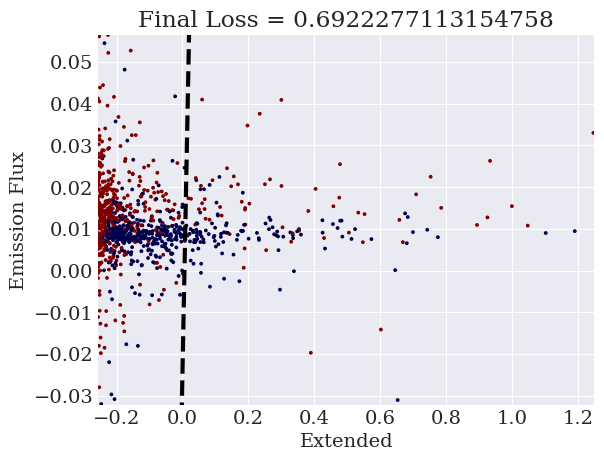
\includegraphics[width=0.48\textwidth]{results/2d_fit_line_minim_extended_emission_flux.png}
    \caption{Distributions of each combination of features with the outer 2\% cut out due to outliers. Black dashed lines indicate the decision boundary of a classification algorithm trained with logistic regression and line minimization using golden section search. The titles indicate the converged loss value.}
    \label{fig:2d_line_minim_scatter}
\end{figure}

In the last panel, corresponding to the combination with the highest loss, we can see that the two classes are very much intertwined making it very difficult for the algorithm to separate the two. The figure also shows us why the combination of color and $\kappa_{\mathrm{CO}}$ work well together to predict the galaxy class. The two classes appear quite clearly as two distinct clusters with only a little bit of overlap in the center. The model attempted to draw its decision boundary between these two clusters, although visually it looks like the true best decision boundary might have been placed slight more to the bottom left. 

To investigate these results quantitatively we also compute the confusion matrix and the F1 score for each of these fits. The F1 score is defined as

\begin{equation}
    \mathrm{F1} = \frac{2 \times \mathrm{precision} \times \mathrm{recall}}{\mathrm{precision} + \mathrm{recall}}
\end{equation}

With 

\begin{align}
    \mathrm{precision} &= \frac{\mathrm{TP}}{\mathrm{TP}+ \mathrm{FP}} \\
    \mathrm{recall} &= \frac{\mathrm{TP}}{\mathrm{TP} + \mathrm{FN}} 
\end{align}

Both the precision and the recall are values between 0 and 1. Therefore the F1 score is also always a value between 0 and 1, where higher numbers correspond to better predictions. We calculate these values for all combinations of features, and present the results in Table \ref{tab:f1_scores}.

\begin{table}[h]
    \centering
    \begin{tabular}{|l|c|c|c|c|c|}
    \hline
    Features & TN & TP & FN & FP & F1 \\
    \hline
    \input{results/confmat_tab_line_minim.txt}
    \end{tabular}
    \caption{Confusion matrix values laid out horizontally and the F1 score computed using these for each combination of two features.}
    \label{tab:f1_scores}
\end{table}

Correspondingly to what we can see both in the loss values and visually, the first combination performs best and the last model performs worst. The rest of the models all hover around F1 $\sim 0.8$. Interestingly, while most of the predictors appear to be equally bad at recreating the label for elliptical and spiral galaxies, the final model is a lot worse at detecting when a galaxy in its training set is a sprial (positive class, corresponding to the red dots in Figure \ref{fig:2d_line_minim_scatter}). This can also be seen in the last panel of that figure because the decision boundary is placed to the right of the majority of galaxies, and there are a lot of blue (negative class, ellipticals) to the left of it still.



